\newpage

\section{Wettbewerbsanalyse} \label{wettbewerbsanalyse}
Wettbewerbsanalyse

Im Rahmen dieses Projektes haben wir eine Wettbewerbsanalyse durchgeführt, um den Markt nach bestehenden Lösungen zu durchsuchen und unsere Unique Selling Propositions (USP) herausarbeiten zu können. Die Wettbewerbsanalyse wurde nach keiner wissenschaftlichen Methode durchgeführt, es wurden lediglich einige Schlagworte in die Suchmaschine Google eingegeben und die Suchergebnisse analysiert. Als Suchbegriffe wurden die Begriffe aus Tabelle 1 in unterschiedlichen Kombinationen verwendet. 

\caption{table}{Suchbegriffe für die Wettbewerbsanalyse}
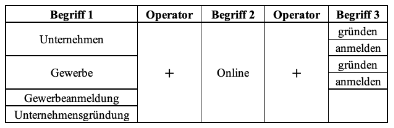
\includegraphics{"chapter/chapter_3/Tabelle 1.png"}
\caption{Quelle: Eigene Darstellung}

Zum Zeitpunkt der Recherche im Januar 2025 konnte kein Anbieter gefunden werden, der eine vollumfassende Unternehmensgründung mit Anmeldung beim Gewerbeamt, Finanzamt, der Prüfung des Unternehmensnamens und einer Eintragung in das Handelsregister anbietet. Allerdings wurden einige Dienstleister gefunden, die bei der Unternehmensgründung unterstützen und einige Teile des Prozesses übernehmen. Die Tabelle 2 gibt einen Überblick über die kommerziellen Anbieter und deren Dienstleistungen, staatliche Institutionen und Behörden wurden nicht berücksichtigt. Bei der Recherche wurden als Bewertungskriterien die Gesellschaftsformen Einzelunternehmen, Gesellschaft mit beschränkter Haftung (GmbH), Gesellschaft bürgerlichen Rechts (GbR), Unternehmensgesellschaft (UG), Aktiengesellschaft (AG) herangezogen.

\caption{table}{Ergebnisse der Wettbewerbsanalyse}
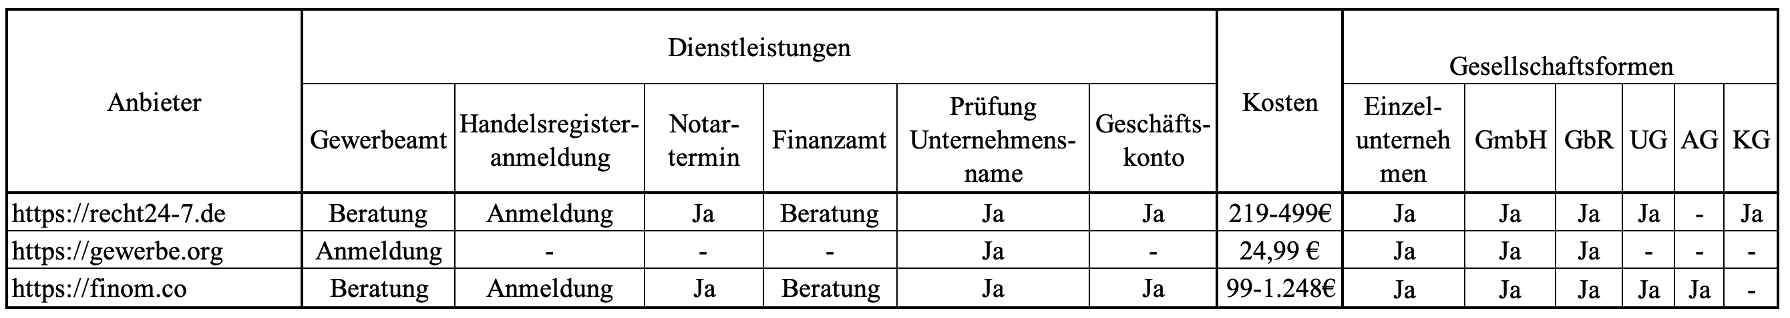
\includegraphics{"chapter/chapter_3/Tabelle 2.png"}
\caption{Quelle: Eigene Darstellung}

Der erste Anbieter, „recht24-7.de“, berät die Kunden zur Anmeldung beim Gewerbeamt und Finanzamt. Die Leistungen umfassen außerdem die Vereinbarung eines Notartermins sowie die Prüfung des Unternehmensnamens und die Anmeldung beim Handelsregister. Auch die Eröffnung eines Geschäftskontos ist in den Leistungen des Anbieters enthalten. Die Kosten des Services liegen je nach Gesellschaftsform zwischen 219 und 499 € und es können eine Vielzahl von Gesellschaftsformen angemeldet werden. \vglfootcite[]{oa_gmbh_nodate}
Der zweiten Anbieter, „gewerbe.org“, bietet lediglich die Beratung und Anmeldung des Gewerbes beim Gewerbeamt an und es können lediglich Einzelunternehmen, Gesellschaften mit beschränkter Haftung (GmbH) sowie Gesellschaften bürgerlichen Rechts (GbR) angemeldet werden. Der Service Kostet 24.99 € (Stand Januar 2025). \vglfootcite[]{oa_unternehmen_nodate}
Der Anbieter „finom.co“ bietet ähnliche Leistungen wie „recht24-7.de“ an. Es werden also die Anmeldung beim Handelsregister sowie die Prüfung des Unternehmensnamens und die Einrichtung übernommen und ein Termin beim Notar vereinbart. Außerdem werden die Gründer hinsichtlich der Anmeldung beim Gewerbeamt und Finanzamt beraten. Auch auf „finom.co“ lassen sich zahlreiche Gesellschaftsformen Gründen unter anderem auch Aktiengesellschaften (AG). Die Kosten des Services sind abhängig von der Gesellschaftsform und liegen zwischen 99€ und 1.248€. \vglfootcite[]{oa_finom_nodate}
Als Fazit ist zu sagen, dass zwei der gefundenen Anbieter ein umfangreiches Gesamtpaket anbieten, allerdings die Anmeldung beim Gewerbeamt und Finanzamt nicht übernehmen und darüber hinaus auch keine Möglichkeit zur Markeneintragung anbieten. Einzig der Anbieter „gewerbe.org“ bietet die Anmeldung beim Gewerbeamt an, allerdings übernimmt dieser keine weiteren Services. Somit konnten wir im Januar 2025 keinen Anbieter in Deutschland identifizieren, der einen allumfassenden Online-Service zur Unternehmensgründung anbietet. 
